\scanpage{72}\mspage{71}

Pour la suite, il faut faire attention si les axiomes vont passer aux sous-contrées. Introduisons quand $= =$ la définition en forme

% R1-FIG-DEFINITION: the raised word and its full hooked connector, with adjoining text once.
\figure{\begin{tikzpicture}[x=1cm,y=1cm]
\node[anchor=west] at (0,0) {\uline{Définition 1} On appelle};
\node[anchor=west] at (7.4,0) {\uline{sous-contrée}};
\node[anchor=west] at (9.4,0.8) {\inserted{[\uline{pleine}]}};
\draw[line width=.55pt] (8.45,.48) .. controls (8.0,.28) and (10.9,.22) .. (11.35,.1) .. controls (11.85,.02) and (11.9,-.12) .. (12.0,-.23) .. controls (12.17,.03) and (12.28,.37) .. (12.31,.55);
\node[anchor=west] at (0,-1.05) {de la contrée $\unsure{\rlap{\deleted{\mathcal F}}\mathcal C|\mathcal C|\mathscr C|\mathbb C}=(\mathcal F,\leq,\preceq)$, \unsure{\deleted{tout}|tout}};
\node[anchor=west] at (0,-1.85) {sous-ens. qui \unsure{satisfait|satisfont} les conditions};
\end{tikzpicture}}

% R1-FIG-A: the two raised insertions and their separate leaders.
\figure{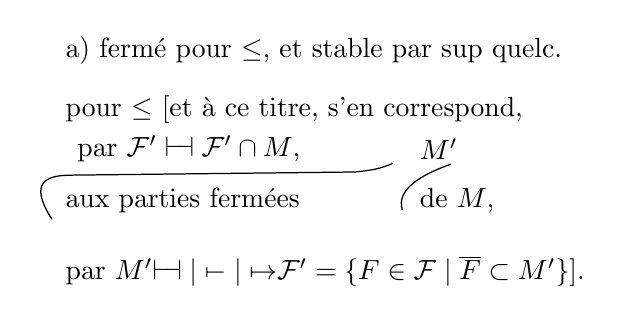
\begin{tikzpicture}[x=1cm,y=1cm]
\node[anchor=west] at (0,0) {a) fermé pour $\leq$, et stable par sup quelc.};
\node[anchor=west] at (0,-.75) {pour $\leq$ [et à ce titre, s'en correspond,};
\node[anchor=west] at (.15,-1.25) {\inserted{par $\mathcal F'\mathrel{\vdash\joinrel\dashv}\mathcal F'\cap M$,}};
\node[anchor=west] at (0,-1.9) {aux parties fermées};
\node[anchor=west] at (4.5,-1.9) {de $M$,};
\node[anchor=west] at (4.5,-1.25) {\inserted{$M'$}};
\draw[line width=.45pt] (-.05,-2.14) .. controls (-.35,-1.67) and (-.13,-1.58) .. (.2,-1.58) -- (3.8,-1.54) .. controls (4.0,-1.52) and (4.12,-1.50) .. (4.28,-1.43);
\draw[line width=.45pt] (4.4,-2.02) .. controls (4.32,-1.77) and (4.62,-1.58) .. (5.02,-1.44);
\node[anchor=west] at (0,-2.8) {par $M'\unsure{\mathrel{\vdash\joinrel\dashv}|\mathrel{\mapstochar\relbar}|\mapsto}\mathcal F'=\{F\in\mathcal F\mid\overline F\subset M'\}$].};
\end{tikzpicture}}

% slanted left margin; the last parenthesis is not securely framed by the one crop.
\margin{Je ne sais s'il faut prendre des sup quelconques (\unsure{condition} stricte) \deleted{\unsure{et}} ou bien de sup finis seulement \unsure{(condition large)|(condition lge)}}

% R1-FIG-B-CORRECTION: replacement above the cancelled clause; crossed/curling mark after M.
\figure{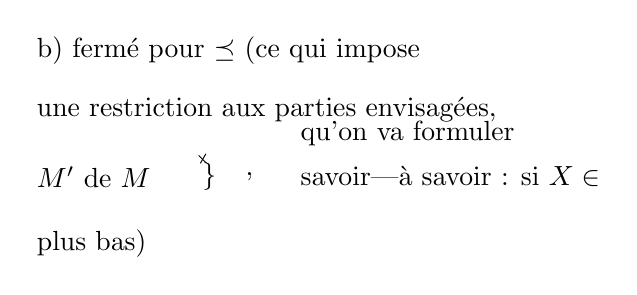
\begin{tikzpicture}[x=1cm,y=1cm]
\node[anchor=west] at (0,0) {b) fermé pour $\preceq$ (ce qui impose};
\node[anchor=west] at (0,-.75) {une restriction aux parties envisagées,};
\node[anchor=west] at (0,-1.6) {$M'$ de $M$};
% R1-MARK-AFTER-M: curled stroke with a small crossing at its head.
\node[anchor=west] at (2.1,-1.6) {\unsure{\}}};
\draw[line width=.35pt] (2.18,-1.33) -- (2.28,-1.43);
\draw[line width=.35pt] (2.20,-1.43) -- (2.27,-1.31);
\node[anchor=west] at (2.65,-1.6) {,};
\node[anchor=west] at (3.35,-1.6) {\deleted{\unsure{savoir|à savoir} : si $X\in$}};
\node[anchor=west] at (3.35,-1.05) {\inserted{qu'on va formuler}};
\node[anchor=west] at (0,-2.45) {plus bas)};
\end{tikzpicture}}

% R1-FIG-MARGINAL-C: marginal continuation above C6; labels occur only here.
\figure{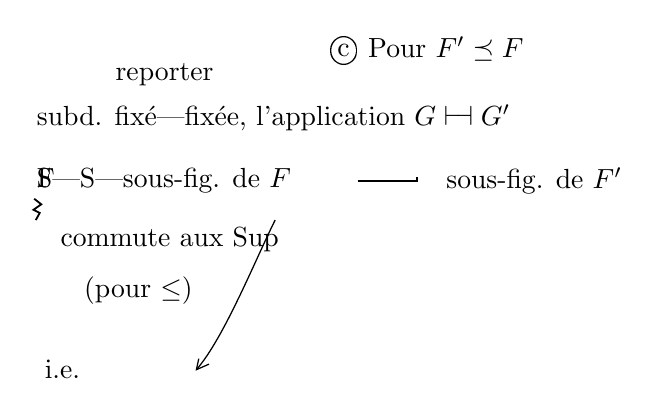
\begin{tikzpicture}[x=1cm,y=1cm]
\node[anchor=west] at (1.0,.55) {reporter};
\node[anchor=west] at (3.7,.85) {\textcircled{c} Pour $F'\preceq F$};
\node[anchor=west] at (0,0) {subd. \unsure{fixé|fixée}, l'application $G\mathrel{\vdash\joinrel\dashv}G'$};
% The worked initial is ONE letter position, including the lower residual strokes.
\node[anchor=west] at (0,-.8) {\unsure{\rlap{\deleted{F}}S|S|s}ous-fig. de $F$};
\draw[line width=.65pt] (.09,-1.03) -- (.18,-1.10) -- (.08,-1.17) -- (.16,-1.21) -- (.11,-1.30);
% R1-C-HEADLESS-LINK: horizontal stroke with a very short raised right endpoint, no arrowhead.
\draw[line width=.6pt] (4.2,-.8) -- (4.95,-.8) -- (4.95,-.75);
\node[anchor=west] at (5.2,-.8) {sous-fig. de $F'$};
\node[anchor=west] at (.3,-1.55) {commute aux Sup};
\node[anchor=west] at (.6,-2.2) {(pour $\leq$)};
\node[anchor=west] at (.1,-3.2) {i.e.};
% A distinct pointer descends leftward from the aux region.
\draw[line width=.45pt] (3.15,-1.3) .. controls (2.9,-1.8) and (2.5,-2.8) .. (2.15,-3.2);
\draw[line width=.45pt] (2.18,-3.06) -- (2.15,-3.2) -- (2.31,-3.13);
\end{tikzpicture}}

% R1-FIG-C6: both literal diagrams, the crossing left rule, the diagonal note, and the right note.
\figure{\begin{tikzpicture}[x=1cm,y=1cm]
\node[anchor=west] at (0,0) {\uline{C6}};
\node[anchor=west] at (2.25,0) {Soit};
% R1-DIAGRAM-FIRST
\node[anchor=north west,inner sep=0pt] at (2.2,-.45) {\begin{minipage}{9cm}
\diagram{\begin{tikzcd}[ampersand replacement=\&,column sep=1.4em,row sep=1em]
F' \arrow[r,phantom,"{\preceq}" description] \& F \arrow[d,phantom,"{\rotatebox{90}{$\leq$}}" description] \& \text{\unsure{de|dans|ds}}~\mathcal F \\
\& G \&
\end{tikzcd}}
\end{minipage}};
% R1-DETACHED-POINTS: two offset small points left of the first diagram.
\fill (2.32,-1.13) circle (.018);
\fill (2.38,-1.18) circle (.018);
% slanted note; the long rule crosses it without cancelling the note.
\node[rotate=42,anchor=south west,align=left] at (-2.05,-2.45) {sym\unsure{e|é}trique\\en $\leq,\preceq$};
\draw[line width=.45pt] (-.15,-.22) .. controls (-.12,-1.4) and (-.12,-4.5) .. (.0,-5.45);
\fill (-.22,-2.1) circle (.013);
\node[anchor=west] at (0,-3.1) {\textcircled{a} Alors il existe un unique $H\in\mathcal F$ \unsure{ou|avec}};
% R1-DIAGRAM-SQUARE
\node[anchor=north west,inner sep=0pt] at (2.7,-3.55) {\begin{minipage}{4cm}
\diagram{\begin{tikzcd}[ampersand replacement=\&,column sep=1.4em,row sep=1em]
F' \arrow[r,phantom,"{\preceq}" description] \arrow[d,phantom,"{\rotatebox{90}{$\leq$}}" description] \& F \arrow[d,phantom,"{\rotatebox{90}{$\leq$}}" description] \\
G' \arrow[r,phantom,"{\preceq}" description] \& G
\end{tikzcd}}
\end{minipage}};
% R1-C6-B-NOTE: circled b is raised after et, not before it.
\node[anchor=west] at (7.1,-3.65) {et};
\node[anchor=west] at (7.55,-3.35) {\textcircled{b}};
\node[anchor=west] at (8.0,-3.65) {les \unsure{str.tes|strates} de};
\node[anchor=west] at (7.1,-4.35) {$G'$ sont les \unsure{\deleted{S}|S|s}tr\unsure{a|.}tes};
\node[anchor=west] at (7.1,-5.05) {$X'$ de $F'$ telles que};
\node[anchor=west] at (7.35,-5.75) {$X'\ll\unsure{G_n|G_m|G}$.};
\draw[line width=.5pt] (6.85,-3.65) -- (6.9,-6.05);
\draw[line width=.5pt] (6.98,-3.65) -- (7.02,-6.05);
\draw[line width=.55pt] (6.85,-5.70) -- (7.03,-5.82);
\node[anchor=west,align=left,font=\small] at (7.35,-6.45) {Ce compl\unsure{é|\.{e}}ment \unsure{servira}\\plus bas};
\end{tikzpicture}}

On dit que $\unsure{G|\rlap{\deleted{F}}G|E}'$ est la \uline{subd} \uline{de} $G$ induite par la subd $F'$ de $F$, ou que $G'$ est la \deleted{\unsure{sous-fig|sous-fig.}}
% slanted lower-left margin
\margin{sur la sous-figure $\unsure{\rlap{\deleted{F}}G|G|E}$ de $F$}
